\documentclass[a4paper]{exam}

\usepackage{amsmath,amssymb, amsthm}
\usepackage{geometry}
\usepackage{graphicx}
\usepackage{hyperref}
\usepackage{titling}
\usepackage{tikz}
\usepackage{tikz-qtree}
\usepackage{framed}


\usepackage{afterpage}
\usepackage{xcolor}
% \graphicspath{{images/}}


\newtheorem{definition}{Definition}
\newtheorem{theorem}{Theorem}
\newtheorem{corollary}{Corollary}
\newtheorem{axiom}{Axiom}
\theoremstyle{claim}
\newtheorem{claim}{Claim}

% Header and footer.
\pagestyle{headandfoot}
\runningheadrule
\runningfootrule
\runningheader{CS/MATH 113 2025}{Pset 10: Graph}{\theauthor}
\runningfooter{}{Page \thepage\ of \numpages}{}
\firstpageheader{}{}{}

% \printanswers %Uncomment this line

\title{Problem Set 10: Graph}
\author{Blingblong} % <=== replace with your student ID, e.g. xy012345
\date{CS/MATH 113 Discrete Mathematics\\Habib University\\Spring 2025}

\pagecolor{pink}
% \afterpage{\nopagecolor}



\begin{document}
\color{purple}

\begin{center}
  
\includegraphics[width=0.4\textwidth]{Rainbow.png}\\
  \huge{Problem Set 11: More on Graphs}\\

  \Large{CS/MATH 113 Discrete Mathematics}\\
  \Large{Habib University Spring 2025}
\end{center}
% \maketitle    
\section*{Problems}

\begin{questions}
  \question Let $G$ and $H$ be some graphs. Show that $G \cong H \iff \overline{G} \cong \overline{H}$
  \begin{solution}
    % Enter solution here 
  \end{solution}

   \question Show that a vertex $c$ in a connected simple graph $G$ is a cut vertex if and only if there are vertices $u$ and $v$, both different from $c$, such that every path between $u$ and $v$ passes through $c$.
   \begin{solution}
    % Enter solution here 
  \end{solution}
\end{questions}

\begin{center}
  The End

  \qed
\end{center}

\begin{center}
  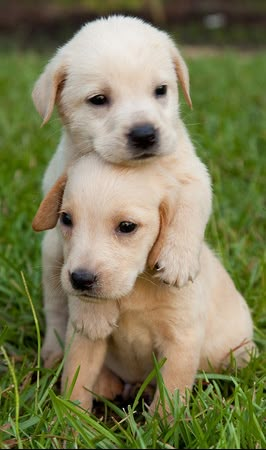
\includegraphics[scale = 0.4]{puppy.jpeg}
  
\includegraphics[scale  = 0.425]{kitten.jpeg}
\end{center}





\end{document}

%%% Local Variables:
%%% mode: latex
%%% TeX-master: t
%%% End:
